\noindent
{
\color{red}
This chapter is intended to evaluate what you did.  The content is highly
topic-specific, but for many projects will have flavours of the following:

\begin{enumerate}
\item functional  testing, including analysis and explanation of failure
      cases,
\item behavioural testing, often including analysis of any results that
      draw some form of conclusion wrt. the aims and objectives,
      and
\item evaluation of options and decisions within the project, and/or a
      comparison with alternatives.
\end{enumerate}

\noindent
This chapter often acts to differentiate project quality: even if the work
completed is of a high technical quality, critical yet objective evaluation
and comparison of the outcomes is crucial.  In essence, the reader wants to
learn something, so the worst examples amount to simple statements of fact
(e.g., ``graph X shows the result is Y''); the best examples are analytical
and exploratory (e.g., ``graph X shows the result is Y, which means Z; this
contradicts [1], which may be because I use a different assumption'').  As
such, both positive {\em and} negative outcomes are valid {\em if} presented
in a suitable manner.
}

Using the automated testing suite to repeatedly run experiments the data
harvested for the next section
was generated by averaging over 30 independant evolution runs
each for 15000 generations. Each test was aimed at evolving circuitry
capable of 2-bit addition (and later 2-bit addition and subtraction). Evaluation
was performed as outlined in the previous chapter; for each of the 16 tests required
for 2-bit addition the binary representation of each number was made available
to the FPGA and after evaluating the circuitry 3 binary values are read off
the bottom of the grid, for each
correct bit the configuration scored 1 point. For both 2-bit addition and weighted 2-bit
addition and subtraction the maximum score is 48.

Much of the published work in genetic algorithm frames maximising the fitness function
as the aim of genetic algorithm parameter choices. Here most of the data harvested
pertains to the accuracy of the configuration; the number of correct bits read off
the FPGA for each test. This is a measure of how good the configuration is, throughout
execution the fitness function simply acts as an incentive to improve this value.

\todo reference back a lot to other papers

All experiments were conducted on a late 2013 15" Apple MacBook Pro with an
Intel Haswell Core i7 processor clocked at 2.3 GHz and 16GB of RAM.

\section{FPGA Simulator}
The main metric by which to judge the quality of the FPGA simulation is the
speed with which a configuration can be instantiated and evaluated.

\todo actually this

\section{Genetic Algorithm Parameter Tuning \label{s:ga_tune}}
All inital genetic algorithm parameters were set mirroring the parameter choice
of \cite{10.1007/3-540-63173-9_61};
a population size of 50, with elitism, linear rank-based selection, the probability
of single point crossover occuring set to 0.7, and the expected mutations per
offspring set as 2.7. However the problem solved in \cite{10.1007/3-540-63173-9_61}
is dramatically different from the addition problem posed here so a great deal
of domain specific tuning is required. This was chosen as the origin of parameter
exploration as it is paper in the existing literiture which has taken the greatest
pains to explain the experiment configuration and setup.

\todo add more explicit parameters to figure
\begin{figure}
	\centering
	\begin{subfigure}[ht]{0.49\textwidth}
		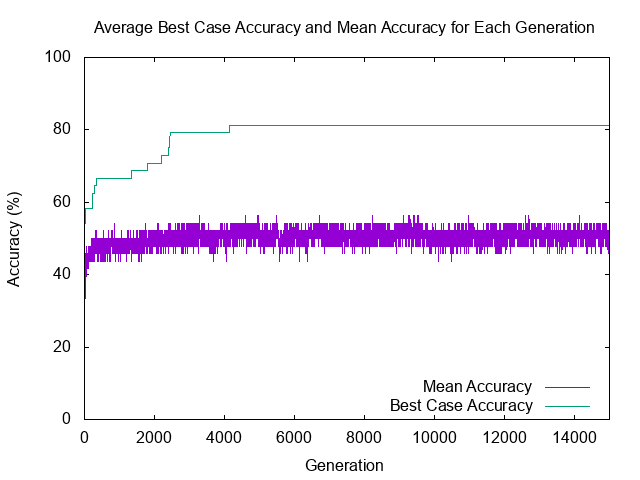
\includegraphics[width=\textwidth]{initial_test.png}
		\caption{}
		\label{fig:initial}
		\vspace{1em}
	\end{subfigure}
	~
	\begin{subfigure}[ht]{0.49\textwidth}
		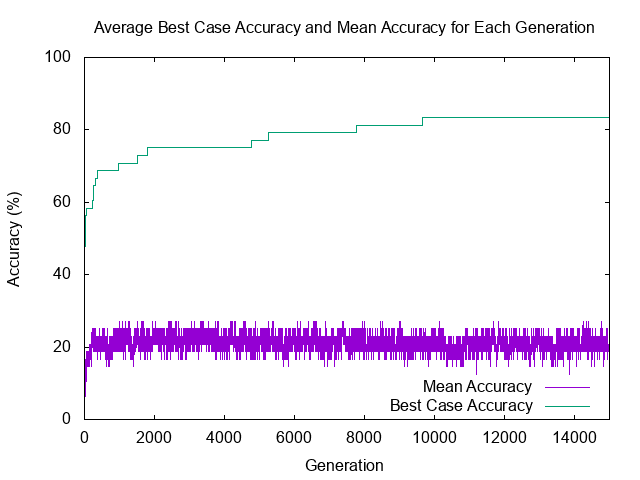
\includegraphics[width=\textwidth]{div_test.png}
		\caption{}
		\label{fig:initial_div}
		\vspace{1em}
	\end{subfigure}
	~
	\begin{subfigure}[ht]{\textwidth}
		\centering
		\begin{tabular}{ccccc}
			\toprule
			& \bfseries{Fitness Function} &
			\bfseries{Perf. Runs (\%)} &
			\bfseries{Avg. Exec. Time (s)} & \bfseries{Avg. Final Accuracy}\\
			\midrule
			(a) & Simple & 0 & 235 & 39\\
			(b) & Multi-Objective & 0 & 267 & 40\\
			\bottomrule
		\end{tabular}
	\end{subfigure}

	\caption[Fitness function test results]{Fitness function test results;
		population size 50, elitism, linear rank-based selection, single point
		crossover probability 0.7, mutation rate 2.7 and
		(a) a simple fitness function mirroring \cite{10.1007/3-540-63173-9_61},
		(b) an extended multi-objective fitness function incorporating a measure
		of diversity with the diversity weight set to 40\% of accuracy.}
\end{figure}

These parameters were evaluated and, as shown in Figure~\ref{fig:initial},
the results of these initial tests are
promising but show a great deal of room for improvement. Despite a healthy
initial improvement in fitness, this quickly reached a plateau and
across the duration of the tests no evolutionary run was
capable of fomulating a perfect solution.
Visual inspection of this initial test as it ran highlighed a huge lack of
diversity in the population of solutions, every improvement in fitness was
an itterative change in the previous best case configuration. This occurs
when a solution improves beyond it's peers and the boost to fertility leads to
it dominating the population. Often a dominating solution will be mostly
correct but due to wildly uneconomic uses of resources be completely incapabale
of evolving any further without dramatic backtracking. The user interface displays
the current average diversity; the distance from one individual to each other in the
population. Relatively early in execution when one member begins to dominate the
diversity plumits.

\todo include proof of plumiting diversity

The diversity in the population averaged (some value), which means that the average number
of different components between an individual and the rest of the population was
as little as 20. With an expected mutation rate of 2.7 this is
indicative of a population completely dominated by a single (potentially bloated)
solution as

\subsection{Improving Diversity}
Such evolutionary
dead ends were also faced by \cite{deJong:2001:RBP:2955239.2955241} who developed
a method of employing multi-objective fitness to encourage population diversity
and minimise waste in solutions. Using their multi-objective fitness function,
a linear combination of diversity and size, to improve the population diversity
and reduce the probability of bloated solutions could provide the evolutionary
pressure required to find a perfect solution. In this situation the final size
of a configuration is inconsiquential, the size is bound to 4x4 and although
a solution which underutilises the FPGA is ideal such stretch goals are beyond
the scope of this document.

A trial was conducted incorporating a diversity measurement weighted at 40\%
of the correctness weighting. This value was arrived at so that diversity,
which exists in the rough range of 0-85, was weighted slightly less than
accuracy, which reaches a maximum of 48.

Figure~\ref{fig:initial_div} dipicts the results from this experiment. Averaged across
repeated executions, there was a slight increase in execution time acompanised by
a marginal improvement in the best case solution fitness
after 15000 generations. However, a larger number of generations was required
to match the accuracy of the simpler fitness function. Despite predictions
to the contrary, another symptom of
the more complex fitness function in this context is a reduced mean population accuracy,
instead of easily beating 20 as happens in Figure~\ref{fig:initial},
\ref{fig:initial_div} maintains a dissapointing
average of 10. This is due to a shift in evolutionary emphasis, in the new
scheme some individuals are given a large fitness due to their novelty alone
and therefore maintained despite their low accuracy, which brings down the
population average. This shift in emphasis also slows the
persuit of perfection; the intial trial in unencumbered with a fitness function
atempting to maintain diversity, and so aggresively persues improvements in
fitness due to a larger proportion of the population which are offspring of a
dominant individual. The slower intial gains in the second trial are indicative
of the smaller segment of the population actively working on the current best
configuration.

These findings disagree somewhat with \cite{deJong:2001:RBP:2955239.2955241},
who found vast improvements across the board when extending the fitness
function. However they did not experiment with population sizes as small
as presented here; unlike our population size of 50, DeJong et al. used
a population size of 1000. It could well be the case that
the population size is too small to facilitate a series of semi-idependently
evolving subpopulations. They also had a mechanism which pruned the population
of ``dominated" individuals which would reduce the tendancy for a population
driven by a fitness function which incorporates diversity to maintain poorly
performing individuals.

To explore this further an experiment with 2 variables was conducted, varying
both the population size (50 and 500) and the incorporation (or not) of a
multi-objective fitness function combining diversity and correctness. A maximum
population size of 500 was used as a
size matching that of DeJong et al. would not feesable in the context as individual
runs would take in excess of 2 hours.

\begin{figure}
	\centering
	\begin{subfigure}[ht]{0.49\textwidth}
		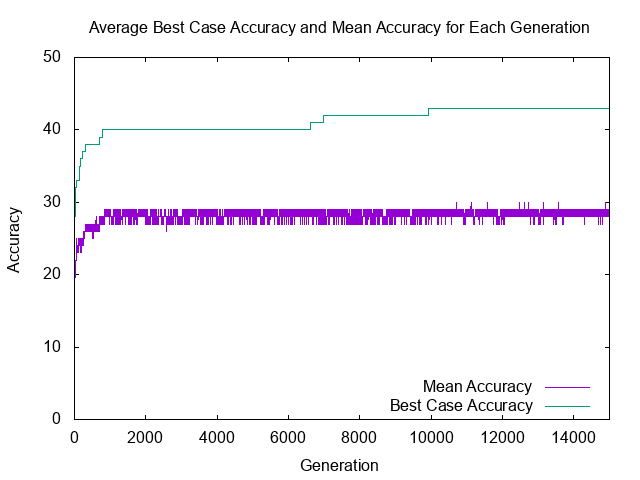
\includegraphics[width=\textwidth]{pop_500_no_div.png}
		\caption{}
		\label{fig:500_no_div}
		\vspace{1em}
	\end{subfigure}
	~
	\begin{subfigure}[ht]{0.49\textwidth}
		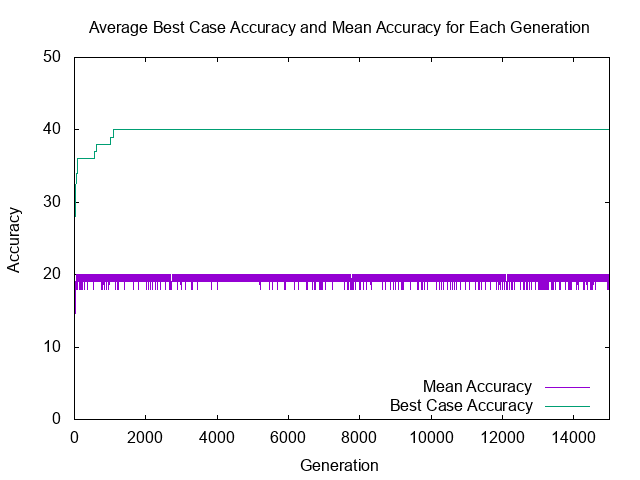
\includegraphics[width=\textwidth]{pop_500_div.png}
		\caption{}
		\label{fig:500_div}
		\vspace{1em}
	\end{subfigure}
	~
	\begin{subfigure}[ht]{\textwidth}
		\centering
		\begin{tabular}{ccccc}
			\toprule
			& \bfseries{Fitness Function} &
			\bfseries{Perf. Runs (\%)} &
			\bfseries{Avg. Exec. Time (s)} & \bfseries{Avg. Final Accuracy}\\
			\midrule
			(a) & Simple & 0 & 2250 & 43\\
			(b) & Multi-Objective & 0 & 2857 & 40\\
			\bottomrule
		\end{tabular}
	\end{subfigure}

	\caption[Large population diversity trail]{Large population diversity trail;
		population size 500, elitism, linear rank-based selection, single point
		crossover probability 0.7, mutation rate 2.7 and
		(a) a simple fitness function mirroring \cite{10.1007/3-540-63173-9_61},
		(b) an extended multi-objective fitness function incorporating a measure
		of diversity with the diversity weight set to 40\% of accuracy.}
	\label{fig:500}
\end{figure}

Figure~\ref{fig:500} contains the results from this experiment. The larger
population size with the simple fitness function (Figure~\ref{fig:500_no_div})
performed the best, the
streamlined persuit of accuracy combined with a larger pool of people to
draw from resulted in the best performance thus far.  The extended function
(Figure~\ref{fig:500_div})
actually reduced the performance, again disagreeing with
\cite{deJong:2001:RBP:2955239.2955241}, and highlighting the
effectiveness of their pruning strategy. This result could be because
the larger population has natural diversity qualities, with a larger pool
a probabilistic procedure such as evolution naturally produces variance,
and the extended
function distracted too much from the persuit of accuracy, and requires a pruning
strategy to reduce waste exploration. The hypothesis
that increasing the population size minimises the reduction in mean accuracy
does ring true. With the smaller population the extended fitness function resulted in
a mean accuracy of less than half the mean accuracy with the simpler fitness function,
whereas
with the a larger population the extended function's trail showed a mean accuracy of
more than
$2/3$rds that of the simpler one.

Despite the improved performance in Figure~\ref{fig:500_no_div} moving forward
further tuning will be performed on the parameters which produced
Figure~\ref{fig:initial_div}. The larger population size in the higher performing experiments
produced an execution time which does not lend itself to exploration and
itterative improvement. Population size will, however, be futher explored in
subsection~\ref{ss:pop_size}.

\subsection{Mutation Rate}

There are two main factors influencing the choice in mutation rate; the fragility
of solutions, and the space between viable individuals. If solutions to a problem are
inherrently fragile, as has been demonstrated in this case by Figure~\ref{fig:landscape},
then a high
mutation rate can regularly destroy working solutions and cause the system to
rarely rise above a fixed value. If the space between viable solutions is vast
a mutation rate which is too small will with low probability cause enough mutations to
span the ravine, yet alone create them in correct places. These two factors are
often at odds, no moreso than in this context, where solutions are brittle and
sparse. Elitism is employed to reduce the impact of fragile solutions by ensuring
the best case solution is never lost, and the inclusion of the extended diversity
fitness function encourages individuals to drift across ravines rather than have
to make the journey in a single step. Therefore the impact of shifting the
fitness function is unclear.

\begin{figure}
	\centering
	\begin{subfigure}[ht]{0.49\textwidth}
		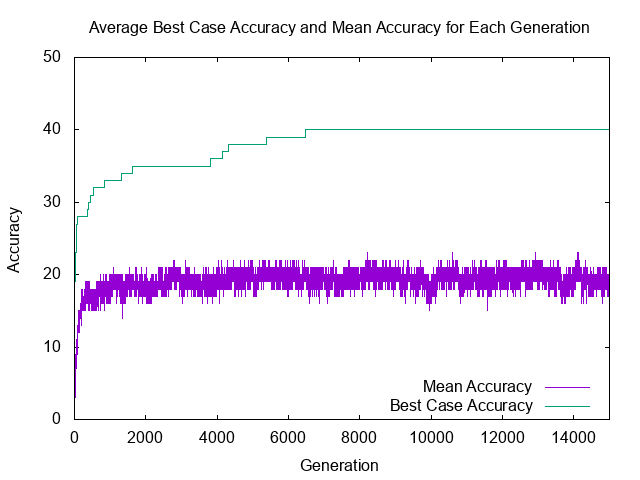
\includegraphics[width=\textwidth]{mut_1.png}
		\caption{}
		\vspace{1em}
	\end{subfigure}
	~
	\begin{subfigure}[ht]{0.49\textwidth}
		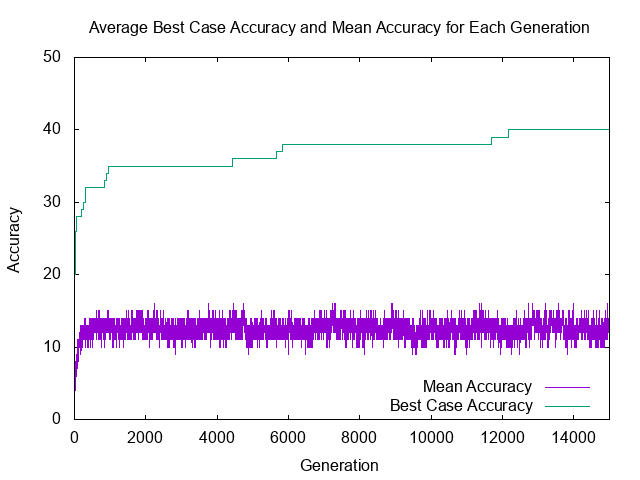
\includegraphics[width=\textwidth]{mut_2.png}
		\caption{}
		\label{fig:mut_2}
		\vspace{1em}
	\end{subfigure}
	~
	\begin{subfigure}[ht]{0.49\textwidth}
		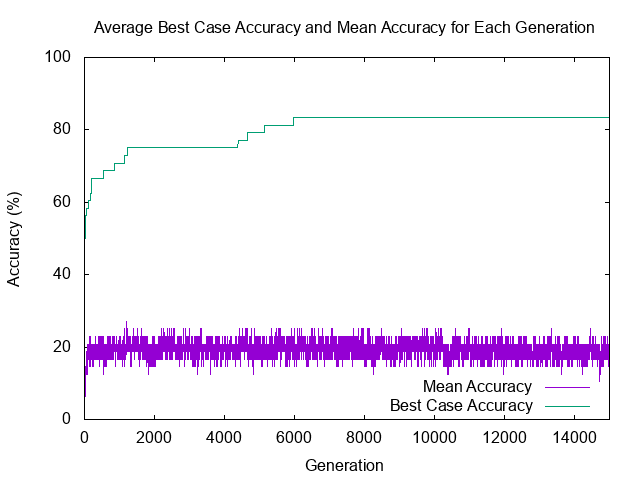
\includegraphics[width=\textwidth]{mut_3.png}
		\caption{}
		\label{fig:mut_3}
		\vspace{1em}
	\end{subfigure}
	~
	\begin{subfigure}[ht]{0.49\textwidth}
		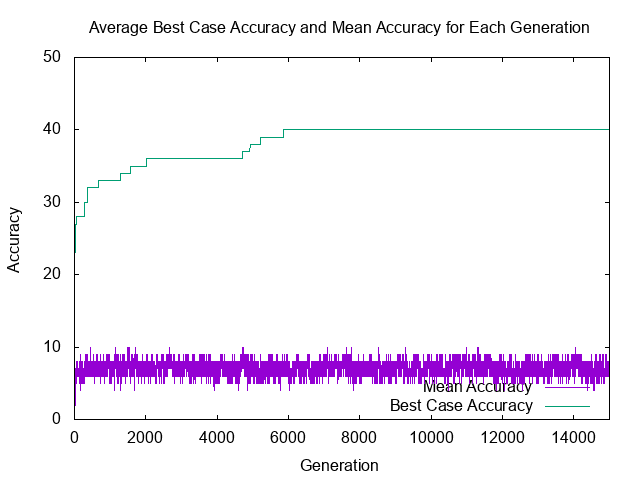
\includegraphics[width=\textwidth]{mut_4.png}
		\caption{}
		\vspace{1em}
	\end{subfigure}
	~
	\begin{subfigure}[ht]{\textwidth}
		\centering
		\begin{tabular}{ccccc}
			\toprule
			& \bfseries{Mutation Rate} &
			\bfseries{Perf. Runs (\%)} &
			\bfseries{Avg. Exec. Time (s)} & \bfseries{Avg. Final Fitness}\\
			\midrule
			(a) & 1 & 0 & 245 & 40 \\
			(b) & 2 & 0 & 264 & 40 \\
			Figure~\ref{fig:initial_div} & 2.7 & 0 & 267 & 40 \\
			(c) & 3 & 0 & 363 & 40 \\
			(d) & 4 & 0 & 368 & 40 \\
			\bottomrule
		\end{tabular}
	\end{subfigure}

	\caption[Mutation rate test results]{Mutation rate test results;
		population size 50, elitism, multi-objective fitness function with diversity
		weighting 40\% of the accuracy, linear
		rank-based selection, single point
		crossover probability 0.7, and
		(a) 1 expected mutation per individual,
		(b) 2 expected mutations per individual,
		(c) 3 expected mutations per individual, and
		(d) 4 expected mutations per individual.}
	\label{fig:mut}
\end{figure}


The experiments conducted in Figure~\ref{fig:mut} mostly agree with the findings
in \cite{10.1007/3-540-63173-9_61} with respect to the experimental results indicating
and ideal mutation rate of around 2.7. However a slight accuracy increase in the
best case individual is
observed when shifting the mutation rate from 2.7 (Figure~\ref{fig:initial_div})
to 3 (Figure~\ref{fig:mut_3}). This is another example of domain specific experimental
tuning for the binary arthmatic problem. The drastic reduction in the speed with which
the best case individual is evolved occuring with a mutation rate of 2
(Figure~\ref{fig:mut_2}) is unexpected. This result could be due to the underlying
topography of the solution landscape; viable solutions are rarely 2 changes apart,
and are more frequently distanced at 1, 3, or 4 changes. This would explain this
marginal reduction in evolutionary swiftness. Note the continuous decrease in population mean accuracy
as the mutation rate is increased, the reasons are twofold; firstly, a higher mutation
rate is more likely to induce a change in an accuracy-critical component of the
solution. Secondly, with an extended fitness function maintaining solutions for
novelty value alone, the more aggresive mutation rate is more likely to cast members of the
population into even further unexplored corners of the fitness landscape giving them
an even higher diversity score (and therefore improving their fitness and their staying power),
these solutions can survive without a high accuracy score.

Because of the results demonstrated by Figure~\ref{fig:mut_3}, namely slighly
improved best-case evolution (at the cost of population accuracy), an expected
mutation rate of 3 has been chosen. This was selected over the mutation rate 1
as the higher population accuracy is a symptom of a more localised less varied
population which is cultivated by a gentler mutation rate.

\subsection{Selection Mechanisms}
The most popular selection methods in evolvable hardware by a considerable margin are
rank selection and tournament selection. Thus far we have been using linear
rank selection (mirroring \cite{10.1007/3-540-63173-9_61}). Here the use
of a variable skewed rank selection is emplyed to place higher evolutionary pressure
on the better performing individuals. The variable controlling the linearity
of the selection function can be set such that the probability of selection
grows quadratically rather than linearly as you move up the rankings. To this
end experiments setting this value to 0 (a quadratic selection function with no linear
component), 0.5, and 1
(completely linear) will highlight any impact this has on the system.

Along with this variation, an experiment comparing current best
selection with tournament selection of varying sizes from 10 (20\% the population
size) upto 40 (80\% the population size). The smaller tournament size
will discriminate less against lower performing individuals, and the
larger the tournament the fewer poorly performing configurations will
be selected for the next generation. This interplay could dramatically
increase performance, exploiting a balance (\todo much like cite cite cite)
to drastically improve performance.

\begin{figure}
	\begin{minipage}{\textwidth}
	\centering
	\begin{subfigure}[ht]{0.32\textwidth}
		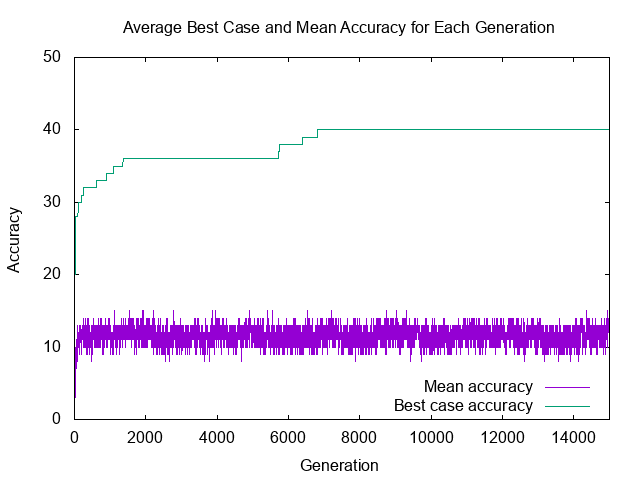
\includegraphics[width=\textwidth]{skew_0.png}
		\caption{}
		\label{fig:skew_0}
		\vspace{1em}
	\end{subfigure}
	~
	\begin{subfigure}[ht]{0.32\textwidth}
		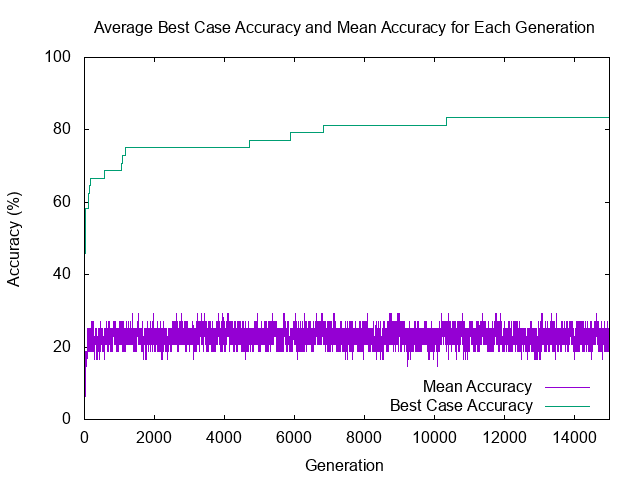
\includegraphics[width=\textwidth]{skew_point5.png}
		\caption{}
		\label{fig:skew_point5}
		\vspace{1em}
	\end{subfigure}
	~
	\begin{subfigure}[ht]{0.32\textwidth}
		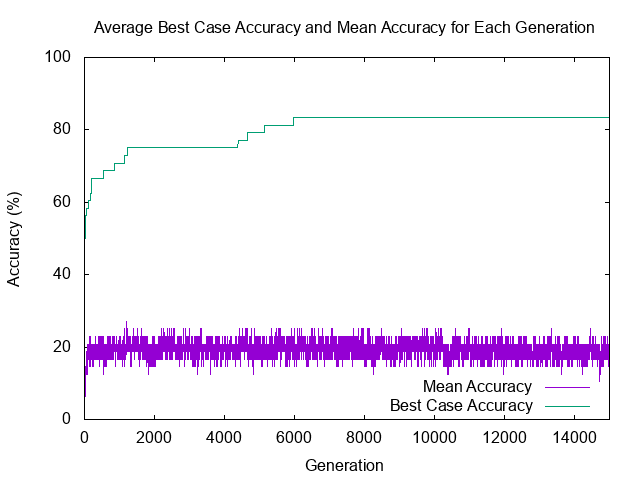
\includegraphics[width=\textwidth]{mut_3.png}
		\caption{}
		\label{fig:skew_1}
		\vspace{1em}
	\end{subfigure}
	~
	\begin{subfigure}[ht]{0.49\textwidth}
		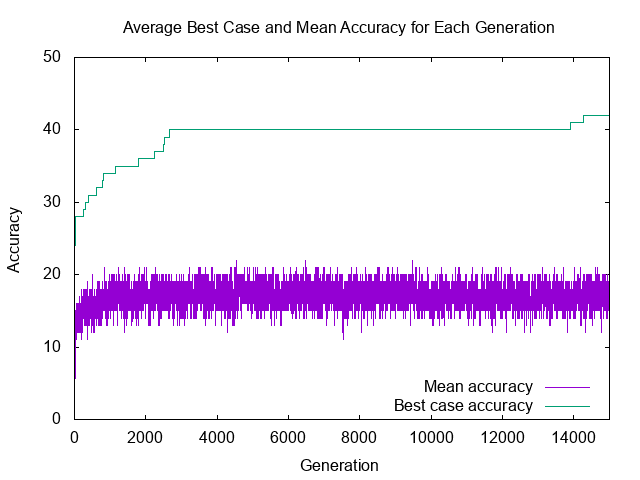
\includegraphics[width=\textwidth]{tour_10.png}
		\caption{}
		\label{fig:tour_10}
		\vspace{1em}
	\end{subfigure}
	~
	\begin{subfigure}[ht]{0.49\textwidth}
		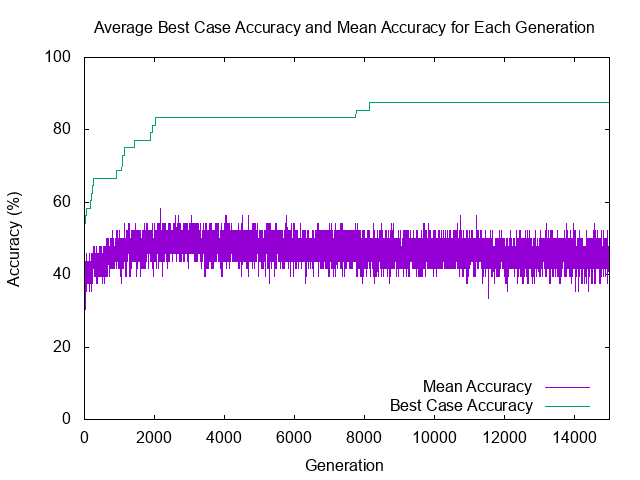
\includegraphics[width=\textwidth]{tour_20.png}
		\caption{}
		\label{fig:tour_20}
		\vspace{1em}
	\end{subfigure}
	~
	\begin{subfigure}[ht]{0.49\textwidth}
		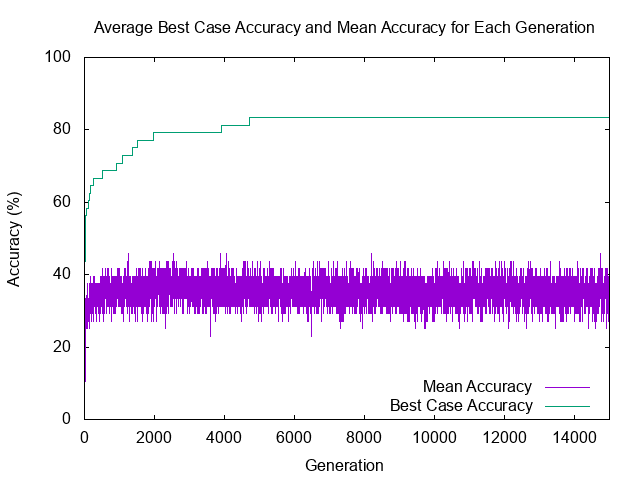
\includegraphics[width=\textwidth]{tour_30.png}
		\caption{}
		\label{fig:tour_30}
		\vspace{1em}
	\end{subfigure}
	~
	\begin{subfigure}[ht]{0.49\textwidth}
		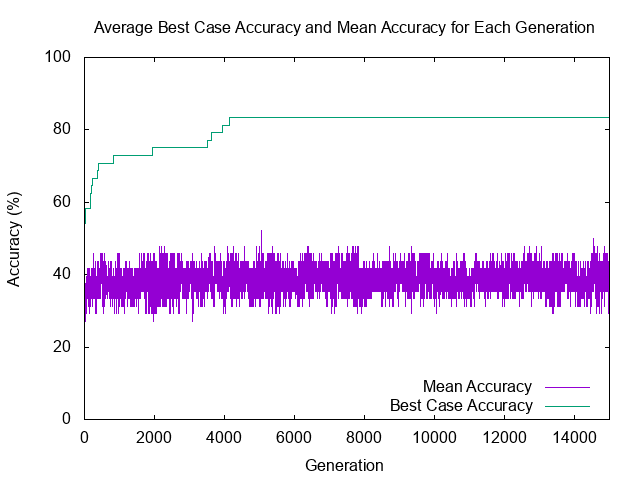
\includegraphics[width=\textwidth]{tour_40.png}
		\caption{}
		\label{fig:tour_40}
		\vspace{1em}
	\end{subfigure}
	~
	\begin{subfigure}[ht]{\textwidth}
		\centering
		\begin{tabular}{ccccc}
			\toprule
			& \bfseries{Selection Method} &
			\bfseries{Perf. Runs (\%)} &
			\bfseries{Avg. Execution Time (s)} & \bfseries{Avg. Final Fitness}\\
			\midrule
			(a) & Rank (Skew 0.0) & 0 & 304 & 40 \\
			(b) & Rank (Skew 0.5) & 0 & 415 & 40 \\
			(c) & Rank (Skew 1.0) & 0 & 363 & 40 \\
			(d) & Tournament (Size 10) & 0 & 264 & 42 \\
			(e) & Tournament (Size 20) & 13 & 231 & 42 \\
			(f) & Tournament (Size 30) & 3 & 260 & 40 \\
			(g) & Tournament (Size 40) & 0 & 244 & 40 \\
			\bottomrule
		\end{tabular}
	\end{subfigure}

	\caption[Selection method test results]{Selection method test results;
		population size 50, elitism, multi-objective fitness function with diversity
		weighting 40\% of the accuracy, single point
		crossover probability 0.7, mutation rate 3 and
		(a)(b)(c)\footnote[1]{(c) duplicated from Figure~\ref{fig:mut_3} for better direct
	visual comparison} rank based
	selection with skew 0.0, 0.5, and 1.0 respectively
	, and (d)(e)(f)(g) using tournament selection with tournament
	size 10, 20, 30, and 40 respectively.}
	\label{fig:select}
\end{minipage}
\end{figure}

The more aggresive discrimination against members of the population due to the
variable skew is clear in Figure~\ref{fig:select}. The population under the more
aggressive selection mechanism (Figure~\ref{fig:skew_0}) persue the
maximum accuracy somewhat quicker than the more linear rank selections
(Figure~\ref{fig:skew_point5} and Figure~\ref{fig:skew_1}), however this
more aggressive discrimination frequently directs the population
with something approaching single-minded determination, often to it's detriment.
The average final fitness is clearly lower with a quadratic rank than with a
linear rank.

Tournament selection with a tournament size of 20 is a clear improvement over
any other selection methods thus far, and has had the single largest impact
on the number of perfect solutions evolved of any parameter choice until
now. 13\% of the trails ended in a perfect solution with an accuracy score of 48.
Individuals are chosen uniformally at random for a tournament, but within a
tournament only the most fit individual wins. This interplay between minimally
and maximally discrimanatory selection schemes results in heavily directed evolutionary
search which maintains a very diverse population. Each of the tournament schemes
have a high population accuracy with a wider variance than any of the rank
selection schemes, indicating the diversity maintainance. The smaller tournament
size, Figure~\ref{fig:tour_10} is too random and does not put enough evolutionary
pressure on finding an accurate solution.
Despite maintaining a broad population the fitness is lower due to this lack of
pressure. The larger tournament size Figure~\ref{fig:tour_40} discriminates too
aggressively, in any selection round the weakest 80\% of the population cannot
be selected (as they are guaranteed to lose the tournament), this leads to a
dominated and ultimately weaker population.
Balancing these two facets of tournament selection, a tournament size
of 20 allows for a search procedure directed enough to find optimal solutions
and with enough random influence to maintain a wide population.

\todo cite tournament selection with binary arithmatic problem

\subsection{Crossover}
Crossover works well in this context, the nature of the mapping between genotype
and phenotype means any crossover can provide benifits to both mating pairs and
inject some much needed diversity into the ecosystem. Three additional trial runs
were execuited, each at a different crossover probability rate; 0, 0.5, and 1.
Crossover points only occur between bytes, never inside them; so
when genetic material is transplanted it is always clean and individual cell
operation is consistent before and after.

\begin{figure}
	\centering
	\begin{subfigure}[ht]{0.49\textwidth}
		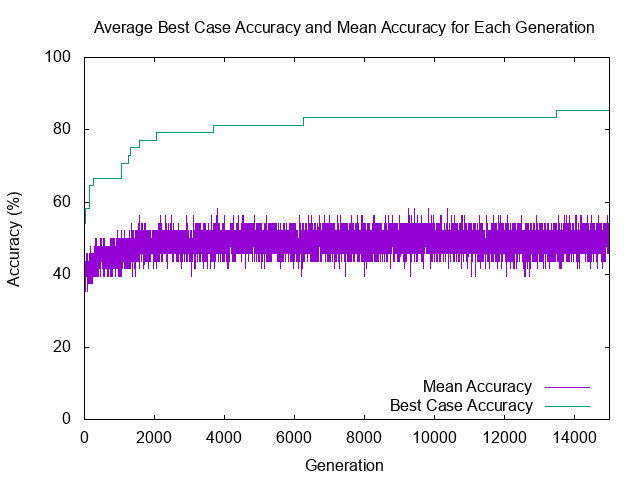
\includegraphics[width=\textwidth]{cross_0.png}
		\caption{}
		\label{fig:cross_0}
		\vspace{1em}
	\end{subfigure}
	~
	\begin{subfigure}[ht]{0.49\textwidth}
		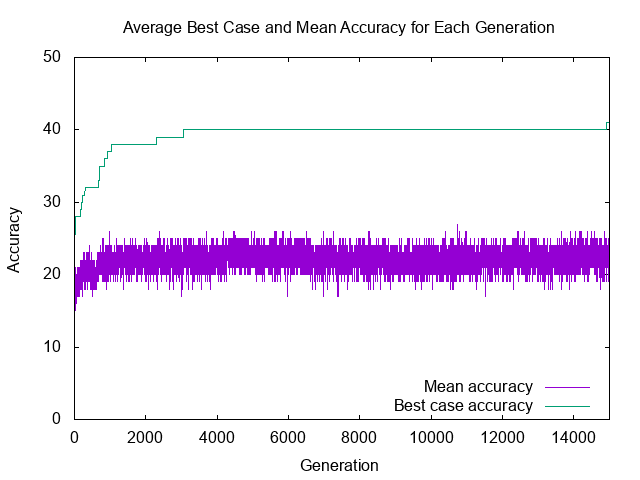
\includegraphics[width=\textwidth]{cross_point5.png}
		\caption{}
		\label{fig:cross_point5}
		\vspace{1em}
	\end{subfigure}
	~
	\begin{subfigure}[ht]{0.49\textwidth}
		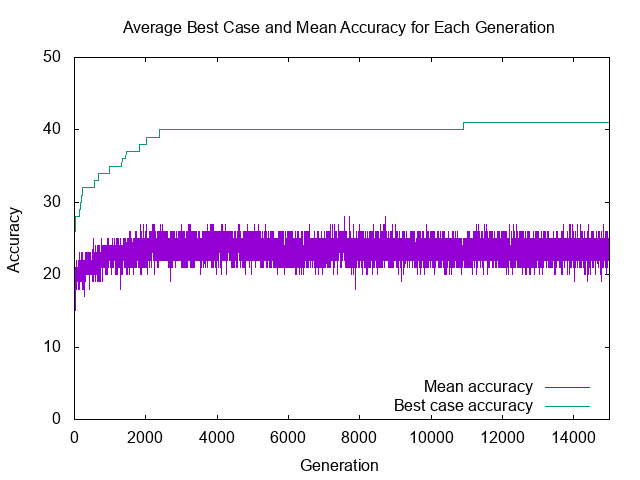
\includegraphics[width=\textwidth]{cross_1.png}
		\caption{}
		\label{fig:cross_1}
		\vspace{1em}
	\end{subfigure}
	~
	\begin{subfigure}[ht]{\textwidth}
		\centering
		\begin{tabular}{ccccc}
			\toprule
			& \bfseries{Crossover Prob.} &
			\bfseries{Perf. Runs (\%)} &
			\bfseries{Avg. Exec. Time (s)} & \bfseries{Avg. Final Fitness}\\
			\midrule
			(a) & 0.0 & 10 & 243 & 41\\
			(b) & 0.5 & 3 & 245 & 41\\
			Figure~\ref{fig:tour_20} & 0.7 & 13 & 231 & 42 \\
			(c) & 1.0 & 3 & 249 & 41\\
			\bottomrule
		\end{tabular}
	\end{subfigure}

	\caption[Crossover probability experiment]{Crossover probability experiment;
		population size 50, elitism, multi-objective fitness function with diversity
		weighting 40\% of the accuracy, mutation rate 3, tournament selection of size
		20, and probability of single point crossover set to (a) 0.0, (b) 0.5, and (c) 1.0.}
	\label{fig:cross}
\end{figure}

In Figure~\ref{fig:cross}, none of the trails produced results rivaling the
initial crossover probability
of 0.7. This behaviour could be a result of how crossover influences the underlying
population structure; never performing crossover and usually performing crossover
performed better than always performing crossover an performing or not with an equal
probability. An explination for the performance at 0 probability could be that
when the population develops without the threat of crossover there is an implicit
encouragement to diversify as there is no punishment for creating a novel solution
which crossover would destroy by mating with an uncompatible partner. Poor performance
at equal probabilities could be a symptom of the same behaviour; when crossover
may or may not happen with equal probabilities a population cannot adapt either way.
The poor performance at 100\% probability would seem to disagree with this, unless you
consider that crossover is ultimately a disruptive force. When crossover is guaranteed
the population can only develop solutions durable in the face of random string swapping.
0.7 provides a good balance where a population can develop with the assumption of
crossover but there is a chance solutions can develop which rely on crossover not
happening.

\subsection{Elitism \label{ss:elitism}}
With a mutation rate as high as shown here the effect of elitism is hightened.
The probability of a mutation crippling a design is relatively high and so a population
without elitism is prone to climbing the evolutionary ladder just to be cast
down by luck. Binary arithmatic is especially fragile, as demonstrated by Figure~\ref{fig:no_elitism},
where the evolutionary parameters are consistent with our highest performer so far, except
elitism is turned off.

\begin{figure}
	\centering
	\begin{subfigure}[ht]{0.49\textwidth}
		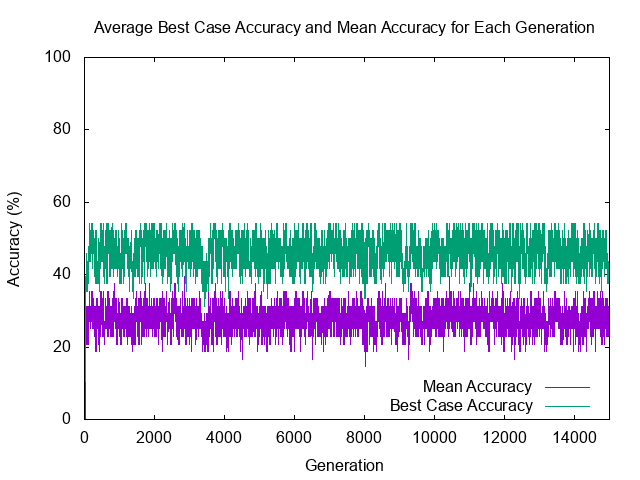
\includegraphics[width=\textwidth]{no_elite.png}
		\vspace{1em}
	\end{subfigure}
	~
	\begin{subfigure}[ht]{\textwidth}
		\centering
		\begin{tabular}{ccc}
			\toprule
			\bfseries{Perfect Solutions (\%)} &
			\bfseries{Avg. Execution Time (s)} & \bfseries{Avg. Final Fitness}\\
			\midrule
			0 & 281 & 19\\
			\bottomrule
		\end{tabular}
	\end{subfigure}

	\caption[Removing elitism test results]{Removing elitism test results;
	population size 50, no elitism, multi-objective fitness function with
	diversity weighting 40\% of the accuracy, mutation rate 3, tournament
	selection of size 20, and probability of single point crossover set to 0.7.}
	\label{fig:no_elitism}
\end{figure}

Clearly, as Figure~\ref{fig:no_elitism} demonstrates removing elitism is crippling.
The population rarely, if ever, performs better than an accuracy of 28. From here
the any path to a better viable solution is insurmountable, crippled by an aggresive
mutation rate, which explored the search space with such vigor that no individuals
performing well can survive due to their inherrent fragility. This dissagrees with
(\todo cite the natural fault tollerence) which claims evolution naturally discoveres
solutions resistant in the face of change; for binary arithmatic the solutions are
too fragile to have such a resistance and require the support of elitism to prop
up the best individuals. Resulting in solutions which do not have the same durability
as a solution found without elitism, if one could ever be found.

\subsection{Tuning Population Size \label{ss:pop_size}}

With the desire to cultivate a diverse population at the forefront of the parameter
selection reasoning enlarging the population would improve the spread of solutions,
and allow the evolutionary pressure on diversity to simultaneously mature and
develop a bredth of solutions.
Obviously increasing the size of the population has objective benifits in a statistical
sense, by casting the net wider there is a higher chance to stumble
accross the correct solution.
But, this has diminishing returns; due to the diversity measurement incorporated into
the fitness function the evalutation time grows with $O(n^2)$ complexity with the
population size.

The increased population size from the experiments with a multi-objective
fitness function could be beyond the point of diminishing returns. To explore this
further trials varying the population size to explore how execution time and
genetic algorithm performance is affected. Population sizes of 25, 50, 100, and 200
were selected to span the bredth of potential choices. For each the tournament size
scaled acordingly, constantly set to 40\% of the whole population (10, 20, 40, and
80 respectively).

\begin{figure}
	\centering
	\begin{subfigure}[ht]{0.49\textwidth}
		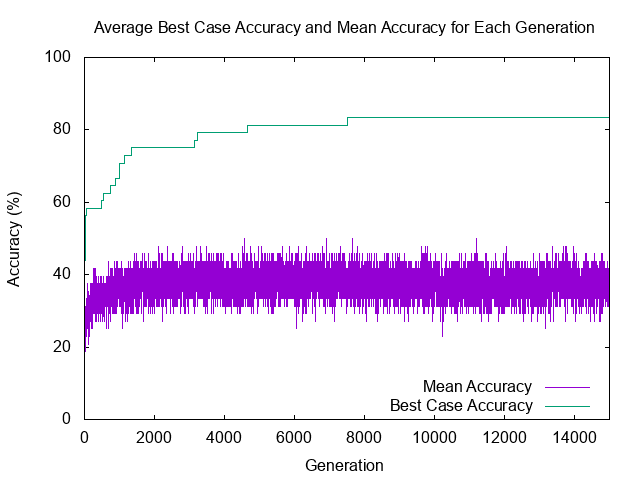
\includegraphics[width=\textwidth]{pop_25.png}
		\caption{}
		\vspace{1em}
	\end{subfigure}
	~
	\begin{subfigure}[ht]{0.49\textwidth}
		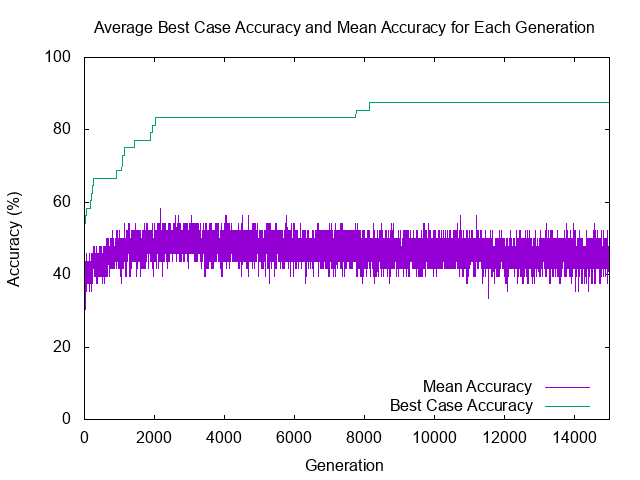
\includegraphics[width=\textwidth]{tour_20.png}
		\caption{}
		\vspace{1em}
	\end{subfigure}
	~
	\begin{subfigure}[ht]{0.49\textwidth}
		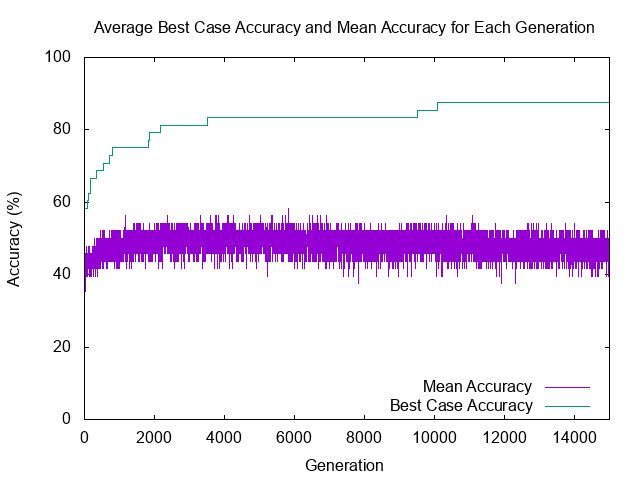
\includegraphics[width=\textwidth]{pop_100.png}
		\caption{}
		\vspace{1em}
	\end{subfigure}
	~
	\begin{subfigure}[ht]{0.49\textwidth}
		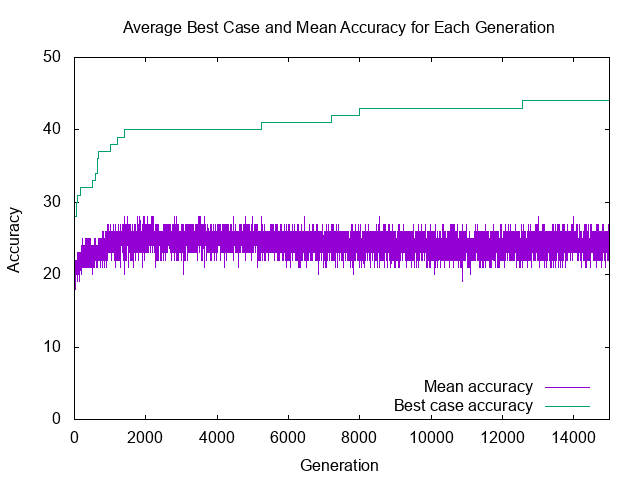
\includegraphics[width=\textwidth]{pop_200.png}
		\caption{}
		\vspace{1em}
	\end{subfigure}
	~
	\begin{subfigure}[ht]{\textwidth}
		\centering
		\begin{tabular}{ccccc}
			\toprule
			& \bfseries{Population Size} &
			\bfseries{Perfect Solutions (\%)} &
			\bfseries{Avg. Execution Time (s)} & \bfseries{Avg. Final Fitness}\\
			\midrule
			(a) & 25 & 0 & 126 & 40\\
			(b) & 50 & 13 & 231 & 42\\
			(c) & 100 & 17 & 457 & 42\\
			(d) & 200 & 57 & 955 & 44\\
			\bottomrule
		\end{tabular}
	\end{subfigure}

	\caption[Population tuning test results]{Population tuning test results;
	elitism, mutli-objective fitness function with diversity weighting 40\%
	of the accuracy, mutation rate 3, tournament selection of size 40\%
	the population size, probability of single point crossover 0.7, and
	(a) population size 25, (b)(duplicated) population size 50, (c) population size 100,
	and (d) population size 200.}
	\label{fig:pop}
\end{figure}

Unsurprisingly the larger population has the highest average final fitness,
and proportion of evolutionary runs ending in a perfect solution but
Figure~\ref{fig:pop} highlights an interesting revelation; Despite the evaluation
function scaling with complexity $O(n^2)$ the increase in execution time is
almost linear with the population. This indicates the poorly scaling portion of
the evalutation function measuring population diversity counts for an insignificant
minority of the execution time. The most aggressive increases in time are due to
the aditional population members which need to be instantiated as FPGAs and
fed the test data. This evidence against the claims made in (\todo ref earlier scaling
claims) demonstrate that the scaling issues are localised to FPGA evaluation.

For all population sizes achieving a best-case accuracy of 36 occured in a
similar amount of time, however the larger populations were able to maintain
this ascent up the evolutionary ladder better. This sudden insummountable
evolutionary barrier for the smaller population sizes implies that the smaller
populations were unable to cultivate a bredth of solutions early in execution
and therefore encountered an evolutionary deadend, temporarily halting improvements.

Moving forward a population size of 50 was selected. Clearly the population size
of 200 is the best candidate, but the increase in persentage of perfect solutions is almost
linear with the added execution time. In order to maintain momentum at this stage
in the project the quicker execution was chosen, with the knowledge that one could
quadrouple the population to increase the execution time and persentage of perfect
solutions by a factor of 4.

\subsection{Tuning Diversity}

One aspect of the evolutionary proccess hitherto unexplored is the relative
weighting given to the diversity measurement in the fitness function. If
set too high the genetic algorithm begins directing for novelty alone,
accuracy is obscured and diversity reigns suprime. If set too low we reenter
the domain of single-minded persuit of accuracy, one which frequently
falls into evolutionary dead ends gracelessly halting progress. Diversity
weighting is defined here as a fraction of the weighting given to accuracy.
Accuracy exists in the range 0-48 for the 2-bit binary arithmatic problem,
and from experimental results diversity usual reaches a maximum value of
around 85. So for any diversity weighting larger than half the size of
the accuracy weighting an individual does well to be maximally diverse,
accuracy occuring as an afterthought. Armed with this knowledge an experiment
was framed running evolutionary
trails at a number of key diversity weightings, 0.0, 0.2, 0.4, and 0.6 accuracy weight.
This shifts evolutionary pressure from completely focussed on accuracy to mostly
completly focussed on diversity.

\begin{figure}
	\centering
	\begin{subfigure}[ht]{0.49\textwidth}
		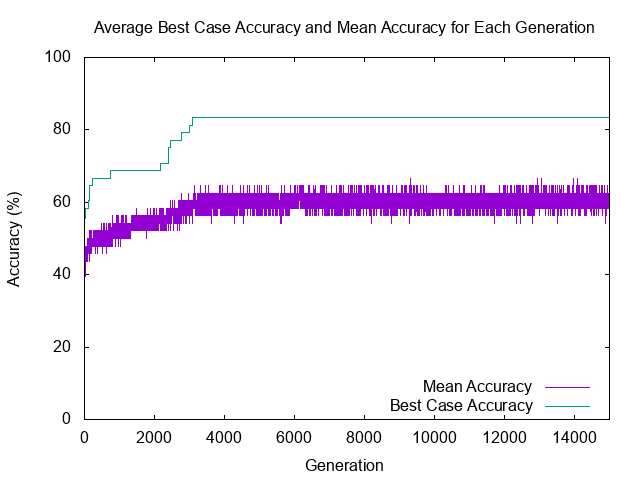
\includegraphics[width=\textwidth]{div_0.png}
		\caption{}
		\label{fig:div_0}
		\vspace{1em}
	\end{subfigure}
	~
	\begin{subfigure}[ht]{0.49\textwidth}
		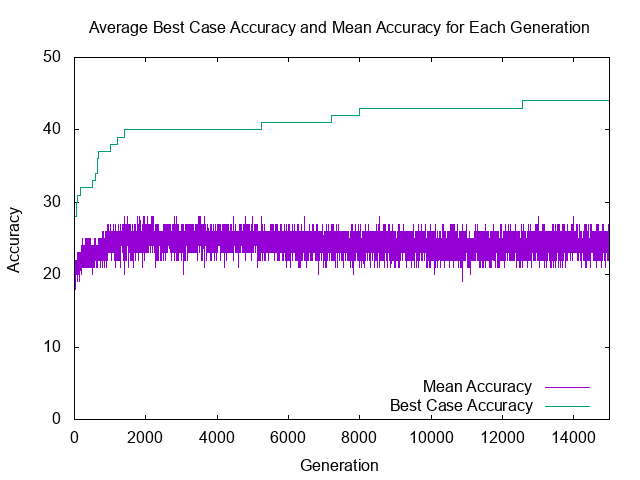
\includegraphics[width=\textwidth]{div_20.png}
		\caption{}
		\vspace{1em}
		\label{fig:div_2}
	\end{subfigure}
	~
	\begin{subfigure}[ht]{0.49\textwidth}
		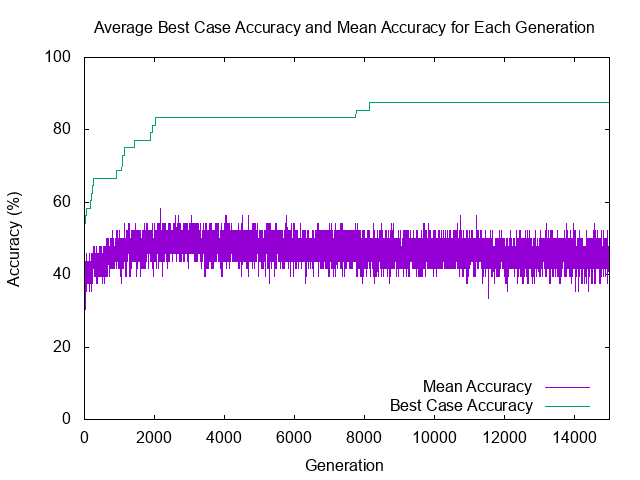
\includegraphics[width=\textwidth]{tour_20.png}
		\caption{}
		\vspace{1em}
	\end{subfigure}
	~
	\begin{subfigure}[ht]{0.49\textwidth}
		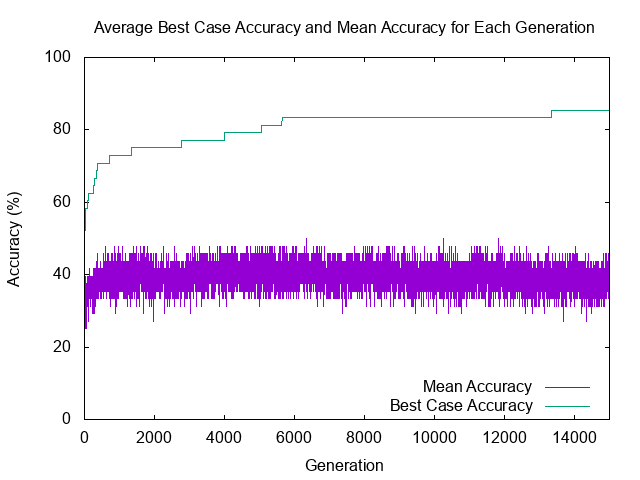
\includegraphics[width=\textwidth]{div_60.png}
		\caption{}
		\vspace{1em}
		\label{fig:div_6}
	\end{subfigure}
	~
	\begin{subfigure}[ht]{\textwidth}
		\centering
		\begin{tabular}{ccccc}
			\toprule
			& \bfseries{Diversity Weighting (\% of Accuracy)} &
			\bfseries{Perf. Runs (\%)} &
			\bfseries{Avg. Execution Time (s)} & \bfseries{Avg. Final Fitness}\\
			\midrule
			(a) & 0 & 16 & 235 & 40\\
			(b) & 20 & 23 & 238 & 44\\
			(c) & 40 & 13 & 231 & 42\\
			(d) & 60 & 10 & 247 & 41\\
			\bottomrule
		\end{tabular}
	\end{subfigure}

	\caption[Diversity weighting test results]{Diversity weighting test results;
	population size 50, elitism, tournament selection of size 20, probability
	of single point crossover 0.7, and a multi-objective fitness function with
	diversity weighting set to (a) 0\%, (b) 20\%, (c) 40\%, and (d) 60\% the weighting
	associated with accuracy.}
	\label{fig:div}
\end{figure}

\todo prune away graphs placed on the same page

Figure~\ref{fig:div} demonstrates the symptoms indicating existing on either side of
balance of power within the fitness fuction between accuracy and diversity. With a
weighting of 0 (Figure~\ref{fig:div_0}) the population hits two evolutionary dead ends,
one at accuracy 34, which it eventually manages to summount and another at accuracy 40
which it fails to improve beyond. The lack of diversity is also clear in the narrow
variance in mean population accuracy. On the other end of the spectrum a weighting of
60\% (Figure~\ref{fig:div_6}) achieved worse perfect solutions but was able to reach
an averge ending accuracy of 41, and all improvements to fitness occured relatively
regularly. This indicates a diverse population with only a small incentive to improve
their accuracy. Balancing this, and improving on the previous best, decreasing the
weighting from 40\% to 20\% seemed to better sit between the two extremes presented
by Figure~\ref{fig:div_0} and Figure~\ref{fig:div_6}.

The reduced effectiveness of diversity at higher weightings is somewhat at odds with
the point of view presented by (\todo cite the multi-objective). As previously mentioned
however their implimentation was coupled with an effective pruning mechanism to dissuade
mindless diversification for the sake of diversification. Also the context each multi-objective
fitness function differs, evolutionary hardware and evolutionary programming are different
animals each with distinct problems. Namely (\todo cite) present theirs as a mechanism
for avoiding the run-away bloat that can happen with evolutionary programming where
the program needlessly gets longer, whereas here we are spacially capped at the size of
the FPGA, looking for a solution within it's confines. It is a subtle difference but
could explain the disparity in results.

\subsection{Coevolution}

Can we exchange the full problem testing system used thus far for a coevolved
parasite population of evolutionarily targeted problems? In order to answer that
question experiments emplying coevolution were conducted on the evolutionary
system developed thus far. Experiments were conducted with a parasite problem
size of 8, 16, and 32; and the best performing parameter choice was repeated
without elitism.

\todo Talk about all the coevolutionary problems from Bullocks paper

\begin{figure}
	\centering
	\begin{subfigure}[ht]{0.49\textwidth}
		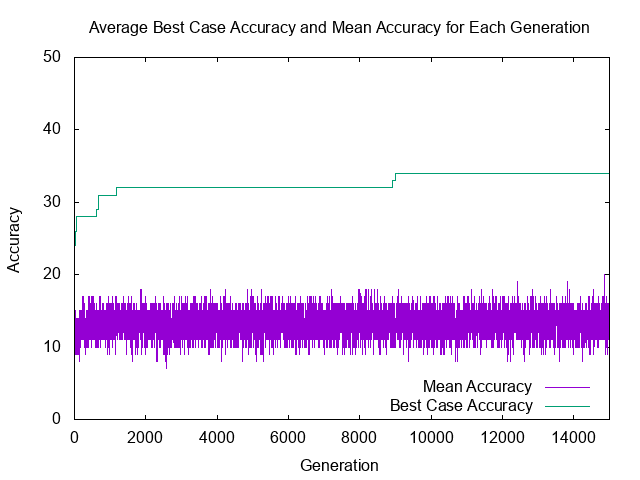
\includegraphics[width=\textwidth]{coev_8.png}
		\caption{}
		\vspace{1em}
		\label{fig:coev_8}
	\end{subfigure}
	~
	\begin{subfigure}[ht]{0.49\textwidth}
		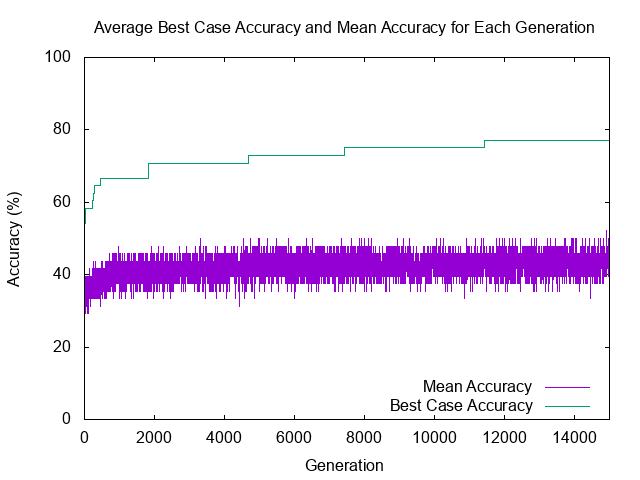
\includegraphics[width=\textwidth]{coev_16.png}
		\caption{}
		\label{fig:coev_16}
		\vspace{1em}
	\end{subfigure}
	~
	\begin{subfigure}[ht]{0.49\textwidth}
		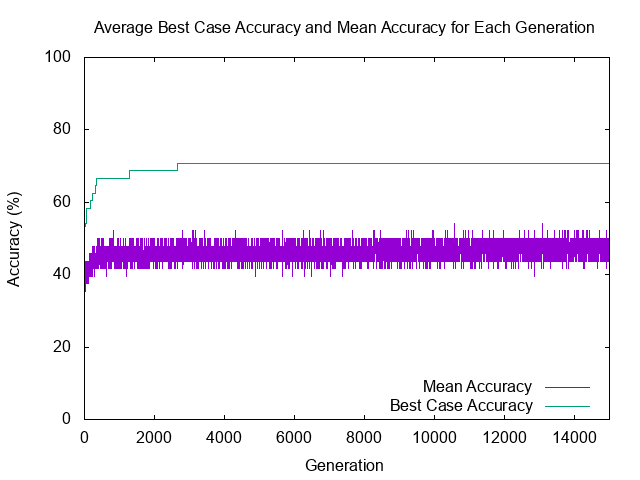
\includegraphics[width=\textwidth]{coev_32.png}
		\caption{}
		\label{fig:coev_32}
		\vspace{1em}
	\end{subfigure}
	~
	\begin{subfigure}[ht]{0.49\textwidth}
		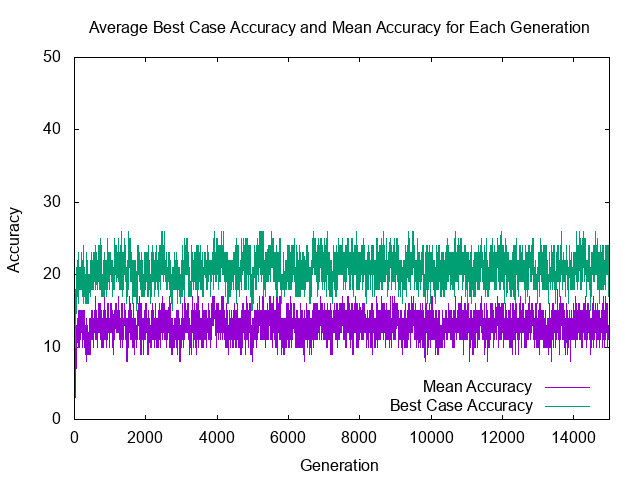
\includegraphics[width=\textwidth]{coev_no_elit.png}
		\caption{}
		\label{fig:coev_16_no_elit}
		\vspace{1em}
	\end{subfigure}
	~
	\begin{subfigure}[ht]{\textwidth}
		\centering
		\begin{tabular}{ccccc}
			\toprule
			& \bfseries{Parasite Size} &
			\bfseries{Perf. Runs (\%)} &
			\bfseries{Avg. Execution Time (s)} & \bfseries{Avg. Final Fitness}\\
			\midrule
			(a) & 8 & 0 & 740 & 34 \\
			(b) & 16 & 0 & 605 & 37 \\
			(c) & 32 & 0 & 703 & 34 \\
			(d) & 16 & 0 & 535 & 24 \\
			\bottomrule
		\end{tabular}
	\end{subfigure}

	\caption[Coevolution test results]{Coevolution test results;
	population size 50, elitism, tournament selection of size 20, probability
	of single point crossover 0.7, a multi-objective fitness function with
	diversity weighting set to 20\%, and a coevolved parasite population where
	each parasite is of size
	(a) 8, (b) 16, and (c) 32 tests. (d) has a parasite consisting of 16 tests
	but elitism is turned off.}
	\label{fig:coev}
\end{figure}

In a coevolutionary system there a series of problems that can disturb the gentle
ballance between host and parasite.
In Figure~\ref{fig:coev} no coevolutionary system was capable of evolving a successful
solution. Each had poor execution time and low final fitness.

Earlier in this document coevolution was touted as a potential solution to the scaling
problem, however comparing Figure~\ref{fig:coev_16} and Figure~\ref{fig:coev_16_no_elit}
it is clear that without elitism the entire system becomes unable to produce a solution
with even somewhat acceptable accuracy. This rehiterates the findings in subsection
~\ref{ss:elitism} in this new context. In order for elitism to have any real impact
with the binary addition problem members of the population have to be exhaustively tested
against all possible problems to allow the elitism metric to keep the best performing
individual regardless of the parasite they are paired against. This disrupts the
notion that coevolution can be used to aid with the scaling issue and will be further
discussed in Section~\ref{s:scaling}. Somewhat surprising is the ability of coevolution
with a parasite which only contains 8 problems (only 4 of which are addition problems)
to provide a semblance of positive evolutionary pressure.

In all the experiments with elitism activated after
a certain amount of time the average population
fitness reaches a plateau and all improvements seem to come from the highest performing
individual(s) with little impact in the overall population. Although similar to
tests not using a coevolutionary system this behaviour could be indicative
of a disengaged population, one in which the parasite population becomes too aggresive
and becomes unbeatable, no longer discriminating in the host population between FPGA
configurations.

\todo Change the virulence

\subsection{Evolved 2-bit addition hardware}

\begin{figure}
	\centering
	
\includegraphics[width=0.45\textwidth]{evolved_adder.png}
	\caption{Successful evolved solution for the 2-bit binary addition problem
	\todo pen and paper test}
	\label{fig:2-bit}
\end{figure}

By now we have a relatively well performing evolutionary hardware system,
tailored directly for the binary arithmatic problem. The tuned parameters
are; population size 50, elitism, tournament selection of size 20,
probability of single point crossover 0.7, and a multi-objective fitness function
with a diversity weight set to 20\% the accuracy weight.
This can be thought of as a modernised, experimentally tuned version of the
parameters used in \cite{10.1007/3-540-63173-9_61}.
With this configuration
the evolutionary process takes, on average 238 seconds to span 15000 generations
and 23\% of executions conclude with a perfect solution to the 2-bit binary addition
problem. One such perfect FPGA configuration is outlined in Figure~\ref{fig:2-bit},
with all superflous components not contributing to the answer manually pruned away.
The graph detailing the average accuracy over time for this parameter choice is Figure
~\ref{fig:div_2}.
This novel solution calculates $b\_0$ in the top right hand corner, and $c$ in the
bottom left, this could well be because crossover encouraged this sort of division
of space and labour. The circuity calculating $b\_1$ is spread throught the device,
highlighting the usefullness of crossover not being a certainty.

With this platform we can explore
a range of uses within the domain of dynamic problems.

\section{Fault Tolerance}

The dynamic problem with the largest immediate impact to consumer and industry
alike is arguably that of a system experiencing faulty behaviour.
With a tuned genetic algorithm, exploration into the capacity to dyanmically
adapt the configuration in the face of such a changed or changing problem provides
the oportunity to thoroughly test evoltionary driven fault recovery and mitigation
strategies.

Using the fault injection framework built into the FPGA simulation, a series
of targeted or randomly generated faults will be introduced to an in-progress
genetic algorithm.

\subsection{Simple Fault Recovery}

By preloading the genetic algorithm with a hand designed 2-bit adder
and then
simulating a highly targeted critical fault within the function of a CLB, insight
can be gained into the capcity of evolvable hardware to act as a fault recovery
system in itself and provide a reliable method of recalibration should a device
experience a fault which would otherwise render it useless.

\begin{figure}
	\centering
	\begin{subfigure}[ht]{0.49\textwidth}
		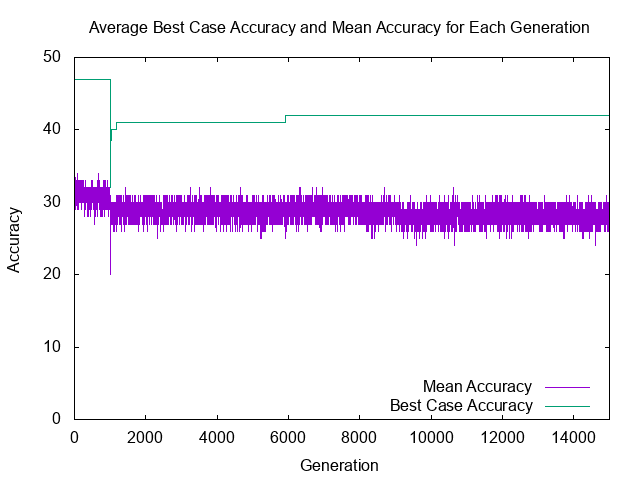
\includegraphics[width=\textwidth]{simple_fault.png}
		\caption{}
		\label{fig:fault}
		\vspace{1em}
	\end{subfigure}
	\\
	\begin{subfigure}[ht]{0.49\textwidth}
		
\includegraphics[width=.9\textwidth]{perfect_adder.png}
		\caption{}
		\label{fig:perf}
		\vspace{1em}
	\end{subfigure}
	~
	\begin{subfigure}[ht]{0.49\textwidth}
		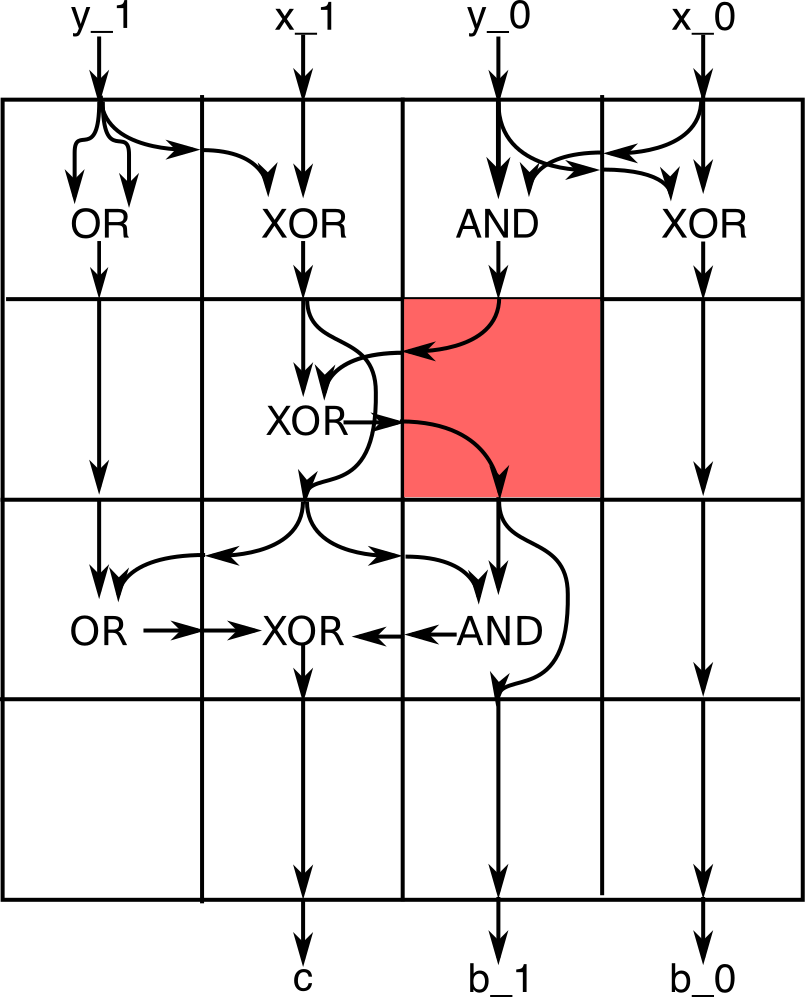
\includegraphics[width=.9\textwidth]{perfect_adder_fault.png}
		\caption{}
		\label{fig:recov}
		\vspace{1em}
	\end{subfigure}
	~
	\begin{subfigure}[ht]{\textwidth}
		\centering
		\begin{tabular}{ccc}
			\toprule
			\bfseries{Perf. Runs (\%)} &
			\bfseries{Avg. Execution Time (s)} & \bfseries{Avg. Final Fitness}\\
			\midrule
			43 & 237 & 42 \\
			\bottomrule
		\end{tabular}
	\end{subfigure}
	\caption[Simple evolutionary fault recovery]{Simple evolutionary fault recovery;
	(a) the accuracy over time, the fault is injected at generation 1000,
	(b) initial preloaded configuration,
	(c) one of the fault mitigation configurations evolved.}
	\label{fig:simple_fault}
\end{figure}

A textbook 2-bit adder was specified, as outlined in Figure~\ref{fig:perf}. The
population was seeded with this adder and the genetic algorithm allowed to operate.
This constitutes the perfect accuracy experienced in Figure~\ref{fig:fault} until generation
1000.
At this point a fault was injected in the CLB shaded red in Figure~\ref{fig:recov}.
This fault clamped the output of the binary function in the cell to an undefined
value and therefore crippled the accuracy of the configuration. The system was then
allowed to evolve as normal in the presence of such a fault.

At 1000 generations, when the fault is injected, the performance drops to levels
well below the regular evolutionary search. However the persentage of executions
ending with a perfect solution is much higher than evolution without the presence
of the fault (Figure~\ref{fig:tour_20}. This could be explained by examining the configuration which seeds
the population; Figure~\ref{fig:perf} performs 2-bit addition using a fraction of the
resources available to the FPGA. Only 7 CLBs are active and all of these are in the top
half of the FPGA. This considerably more compact solution, even with an accuracy score
of only 30, allows the genetic algorithm maximal space to experiment and improve fitness.
Evolutionary deadends are virtually
erradicated by the efficient start point which provides the genetic algorithm a great
deal of flexibility to orchestrate a solution from the bountiful resources.
This leads to frequent perfect recoveries, an even if the solution evolved is not perfect,
there are drastic performance improvements over the faulty chip almost immediately after
the fault occurs.

\todo this framework agrees with \cite{10.1007/3-540-61093-6_6} who deploy EHW when
a fault is detected.

\subsection{``Sticky" Fault Mitigation}
``Sticky" faults occur when certain unpredictable environmental conditions cause
a fault to occur, as such whether or not a fault is active oscilates seemingly at
random. This unpredictablility makes diagnosis and mitigation difficult.
To simulate a sticky fault, randomly generated faults were injected into the simulation,
and activated
or deactivated every 500 generations. 

\begin{figure}
	\centering
	\begin{subfigure}[ht]{0.49\textwidth}
		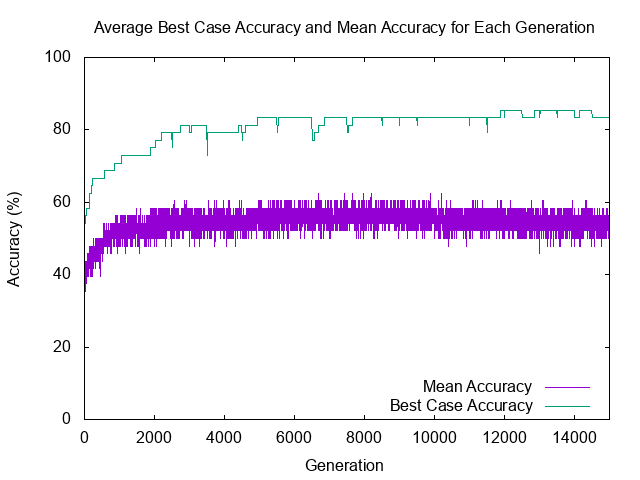
\includegraphics[width=\textwidth]{sticky_1.png}
		\caption{}
		\vspace{1em}
	\end{subfigure}
	~
	\begin{subfigure}[ht]{0.49\textwidth}
		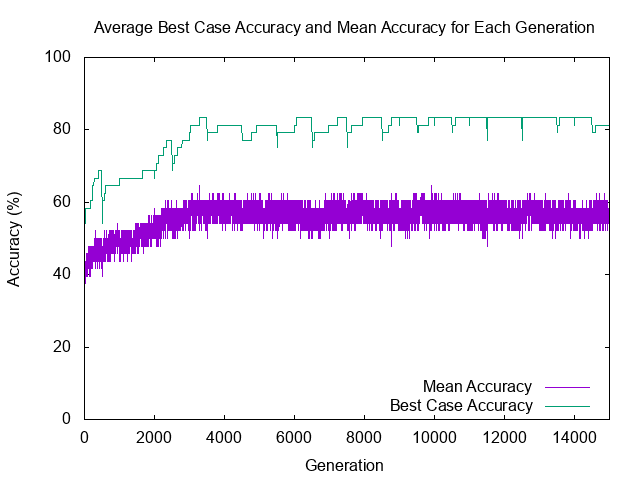
\includegraphics[width=\textwidth]{sticky_2.png}
		\caption{}
		\vspace{1em}
	\end{subfigure}
	~
	\begin{subfigure}[ht]{\textwidth}
		\centering
		\begin{tabular}{cccc}
			\toprule
			\bfseries{Fault(s)} & \bfseries{Perf. Runs (\%)} &
			\bfseries{Avg. Execution Time (s)} & \bfseries{Avg. Final Fitness}\\
			\midrule
			1 & 7 & 242 & 40 \\
			2 & 0 & 230 & 39 \\
			\bottomrule
		\end{tabular}
	\end{subfigure}
	\caption[Evolutionary ``sticky" fault recovery]{Evolutionary ``sticky"
		fault recovery; faults oscilated between on and off every 500
		generations, with
		(a) 1 randomly generated fault and (b) 2 randomly generated
	faults.}
	\label{fig:sticky}
\end{figure}

As one would anticipate the injection of a fault initially has an adverse affect on
accuracy, as is clear in Figure~\ref{fig:sticky}, but eventually the damaging effects
of the fault are lessened. With a single fault 7\% of the evolutionary runs
were capable of evolving a solution which performed perfectly with or without
the fault. There are comparable results with 2 randomly generated faults, despite
never evolving a perfect solution the limitations presented by the faults diminished
over time as the system learned to cope.

The capacity to create solutions from scratch which are resilient to specific faults
is clear. This agrees with \todo cite, who use learned fault models to generate
hardware which can exist in the presence of a fault.

\section{Dynamic Problem Optimisation}
By introducing subtraction as a problem alongside addition, the relative weightings of a correct answer for each problem can be varied to explore dynamically changing problems. In the graph below the genetic algorithm starts with a perfect ADDer and 100\% of the fitness weighting assigned to correct ADDs, every 200 generations this shifts by 10\% towards SUBs.

\begin{figure}
	\centering
	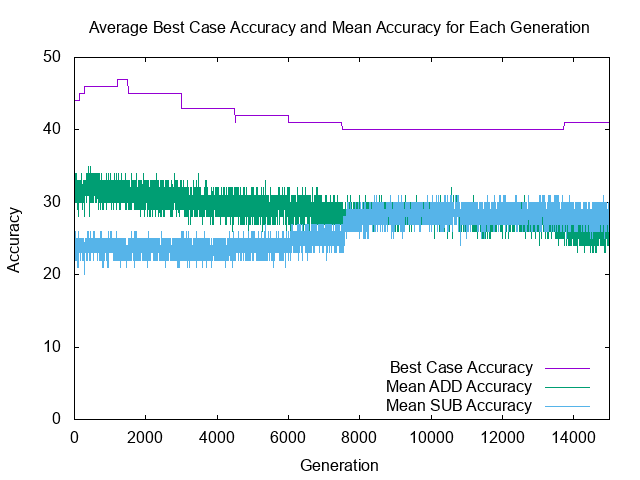
\includegraphics[width=0.49\textwidth]{weighting.png}
	\caption[Accuracy in the presence of dynamic probelm weightings]
	{Accuracy in the presence of dynamic probelm weightings;
		every 1500 generations the accuracy weightings in the fitness
	function shifted 10\% away from ADDs and towards SUBs.}
	\label{fig:weight}
\end{figure}

\todo talk about Figure~\ref{fig:weight}

\section{Scaling \label{s:scaling}}

The poor scaling qualities of evolvable hardware are a known issue, and
unfortunately the system presented here is no different. Initial fears
about the execution time of the evaluation function were assuaged by
the experiments in Figure~\ref{fig:pop}. Despite a diversity measurement
which scales with complexity $O(n^2)$ as the population increases, the
execution time grows linearly. This is because the regions of the algorithm
scaling slowly are minimal and will not reach noticable values until the
population baloons to an unpractical size.

The main culprit for lengthy execution time is clearly therefore the
instantiation and evaluation of FPGAs. Eariler in this document coevolutionary
techniques were toted as a technique to minimise the number of evaluations,
and therefore minimise the FPGA evaluation time; Figure~\ref{fig:coev}
clearly demonstrates data to the contrary. Despite fewer tests in
Figure~\ref{fig:coev_8} and Figure~\ref{fig:coev_16} the execition times
are considerably lengthier than the previous non-coevolutionary searches.
Initially it was thought that the culprit for these poor execution times
was the incorporation of elitism, which relied on conventional scoring
methods to maintain consistent growth in accuracy. Turning this off
resulted in Figure~\ref{fig:coev_16_no_elit}, which despite executing quicker,
performed terribly and was still slower than the conventional evolutionary
counterpart.

An overlooked aspect of the coevolutionary system was the additional computation
required to maintain this second population. This constitutes a huge execution
overhead and ruins any capacity for coevolution to be used as a scaling mitigation
strategy. These trails were, however, only conducted on relatively small problem
sets. The 2-bit addition problem only has 16 trials for addition and 16 trails
for subtraction.

\begin{figure}
	\centering
\begin{tabular}{cccc}
	\toprule
	\bfseries{FPGA Size (Width x Height)} & \bfseries{Exec. Time (s)} & \bfseries{Test Cases}
										  & \bfseries{Exec. Time per Test (s)} \\
	\midrule
	2x4 & 32 & 4 & 8\\
	4x4 & 238 & 16 & 14\\
	6x4 & 1473 & 64 & 23\\
	8x4 & 8537 & 256 & 33\\
	\bottomrule
\end{tabular}
\caption[Execution time for genetic algorithm opperating on different FPGA sizes]
{Execution time (s) for genetic algorithm opperating on different FPGA sizes for
a population of 50 over 15000 generations, the number of test cases is defined
by the width of the FPGA.}
\label{fig:size}
\end{figure}

Further exploring this scaling issue the size of the FPGA was varied.
The evolutionary platform developed in conjunction with this document
defines the scale of the problem being addressed by the size of the FPGA
it is provided with. An FPGA of width $w$ coincides with $\frac{w}{2}$-bit arithmatic.
As such as the size of the FPGA scales in Figure~\ref{fig:size} as does
the problem, and therefor the number of test cases.

The balooning execution time in Figure~\ref{fig:size} highlights that the
scaling issue is domineered by the number of test cases in each problem. A linear increase in FPGA
size from 8 CLBs (2x4) to 32 CLBs (8x4) sees a 267 fold increase in execution
time, but a 64 times increase in the number of test cases each FPGA is evaluated
against. The execution time for each trail scaled slower than the FPGA size.
This clearly identifies the scaling issue as a symptom of the number
of test cases, despite minor growth in evaluation time for larger FPGAs.
As evolvable hardware starts tackling larger and larger
problems coevolution could be used to limit the number of test cases, if the
dramatic performance disadvatages can be overcome. This agrees with \todo cite

Exploring the effects of a growing search space (as the FPGA size increases)
is a well documented issue (\todo cite) beyond the scope of this thesis.
